	\chapter{METHODOLOGY}
	\label{chap:methodology}
	
	This section briefly explains about how the vehicles are classified, how the Travel pattern and Charging/Discharging pattern is formulated and how it is incorporated with `Rtp' to find the best case scenarios. It also explains about the Load profiles took to identify and analyse the 33 bus system and 69 bus system.
	
	\section{Vehicle Classification}
	
	 Electric vehicles have been classified primarily into four major categories as shown in Figure~\ref{fig:classification} 
	 	
			\begin{figure}[h]
				\centering
				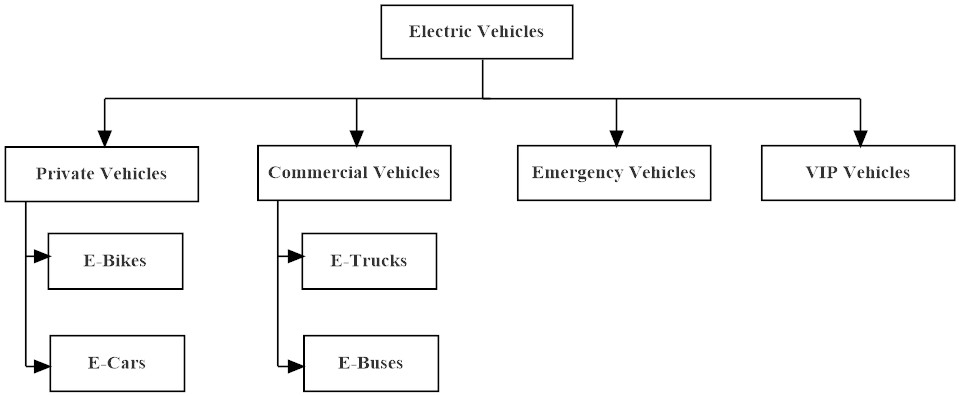
\includegraphics[width=0.7\linewidth]{./Figures/classification}
				\caption{Vehicle Classification}
				\label{fig:classification}
			\end{figure}
		
	The above classification is made by comparing the battery capacity of the vehicles from the data taken with the battery capacity of the similar kind of vehicles in the market.

	\par {Private vehicles are further classified into E-bikes and E-cars with average battery capacity of 400 $Wh$ to 500 $Wh$ and 40 $kWh$ to 100 $kWh$ respectively. Commercial vehicles are classified into E-Truck and E-Bus with an average battery capacity of 100 $kWh$ and 60 to 548 $kWh$ respectively. Emergency vehicles have a battery capacity of around 105 $kWh$ and VIP vehicles have around 90 $kWh$ to 200 $kWh$.
	}
	
	\section{Travel Pattern Establishment}
	
	Travel pattern for three main vehicle subcategories of the above mentioned vehicle categories namely E-car, E-Truck and E-Bus are now taken and travel patterns of the same have been established by using the Battery capacity, Time taken to full charge, Time period of the vehicle when it is connected to the grid , charging rate and discharging rate \cite{evdata}.
	
	Car: ID – 13646 \cite{evdata} is chosen for E-Car as its battery capacity matches with the most common types of E-cars in the market. The
	battery capacity range of this vehicle is 54 $kWh$. The time taken for 100\% charging of battery
	happens to be 1 hour 40 minutes. It then continues to Travel for 6 hour 30 minutes after which the Battery's Charge of the vehicle is depleted. This vehicle is connected to the grid for 5 hours 20 minutes until the next trip. The charging/discharging rate is 10.8 $kW$ per twenty minutes.
	
	Truck: ID – 4428 \cite{evdata} is chosen for E-Truck as its battery capacity matches with the most common types of E-Trucks in the market. The
	battery capacity of this vehicle is 99.2 $kWh$. The time taken for 100\% charging of battery
	happens to be 4 hours. It then continues to Travel for 14 hours after which the Battery's Charge of the vehicle is depleted. This vehicle is connected to the grid for 10 hours until the next trip. The charging/discharging rate is 8.267 $kW$ per twenty minutes.
	
	Bus: Vehicle ID – 16034 \cite{evdata} is chosen for E-bus as its battery capacity matches with the most common types of E-Buses in the market. The
	battery capacity of this vehicle is 199.95 $kWh$. The time taken for 100\% charging of battery
	happens to be 5 hours 20 minutes. It then continues to Travel for 13 hours after which the Battery's Charge of the vehicle is depleted. This vehicle is connected to the grid for 11 hours until the next trip. The charging/discharging rate is 12.5 $kW$ per twenty minutes.
	



	\section{Charging/Discharging Pattern Establishment}
	
	A 24 hour time scale is taken for charging/discharging pattern formulation. This time scale is further subdivided into 72 time blocks as the classified vehicles have non-uniform charging time, thereby rounding of time into hourly basis would be inefficient and unprecise. So inorder to increase precision, the 24 hour scale is split into 72 Blocks.
	
	\noindent Inorder to find the best charging/discharging/idle pattern equation (4.6) is used and this pattern provides less loss to the grid and is useful to the vehicle owner interms of cost.
	
	\noindent After running through all successive time logs of vehicles the whole data is analysed with the equation (4.7) and the connection time which is most profitable for both user and grid is identified.
	
	
	\section{Flowchart}
	
	\begin{enumerate}
		
		\item Data necessary for the EV charging is collected from the device and the time period for which it will be connected to the grid from the user.
		
		\item $SoC_{residual,t}$ is calculated from checking the vehicle's battery.
		
		\item This $SoC_{residual,t}$ is then compared with the $SoC_{threshold,t}$ to determine either to charge or discharge.
		
	
		\begin{enumerate}

			 \item If the SoC is above the Threshold limit there are two viable options either we can discharge or stay idle.
			 

	 	
				 	\item Discharging of the vehicle takes place during peak hours.
					\item Then The Priority score is checked in order to determine whether to charge or keep the vehicle idle. Emergency vehicles and VIP vehicles will have a priority core of `1'.

				
			 \item If the SoC is below the Threshold limit there are two viable options either we can charge or stay idle.
			 
	
			 		\item Charging of the vehicle takes place during off peak hours.
			 		\item If it is an off peak hour and the vehicle needs to charge, we run the vehicle data through a Real Time Pricing Algorithm where the time periods and energy required will be compared with `Rtp' and an efficient pattern of charging is identified (\ref{chap:best}).
			 		

		\end{enumerate}
		
		\item Then the time period is incremented and the process repeats till the time period is the total connection time.
	\end{enumerate}
	
	\begin{figure}
		\centering
		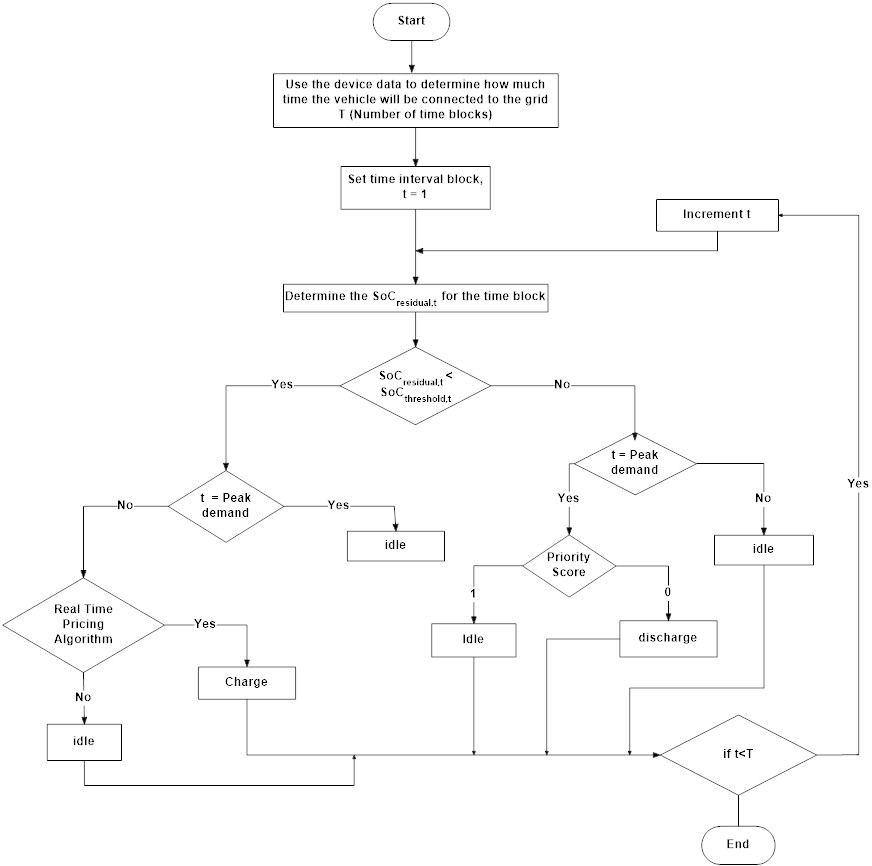
\includegraphics[width=0.9\linewidth]{Figures/Ev_flowchart}
		\caption{Flowchart for Charging/Discharging Pattern}
		\label{fig:evflowchart}
	\end{figure}


	\section{Real Time Price}
		Real Time Price(`$RTP$') is the cost structure in which the cost for per-$kWh$ varies for every hour. Based on `$RTP$' on previous and successive hour it can be decided at which hour the vehicle has to charge, stay idle or to discharge during peak demand. During peak hours it observed that the cost is higher and the vehile can be charged at that time block. 
		
	
		\begin{figure}[!h]
			\centering
			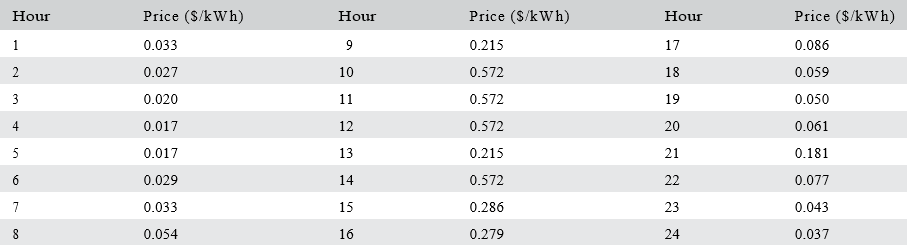
\includegraphics[width=0.7\linewidth]{Figures/rtp}
			\caption{Real Time Price}
			\label{fig:rtp}
		\end{figure}
	
		The product of Charging/Discharging patterns of vehicles (fig \ref{fig:cpcase1} \ref{fig:cpcase2} \ref{fig:cpcase3}) and `$RTP$' are calculated to find the most economical time interval to charge the vehicle. The charge/discharge pattern for each time interval is multiplied correspondingly with the `$RTP$'. The cost for each time interval are cumulatively added together to arrive at the total cost using equation \ref{eqn:bestpattern} and then `$argmin$' function is used to find the lowest or minimum cost using equation \ref{eqn:argmin}. 
	
	
	\section{Load Profile}
		\begin{figure}
			\centering
			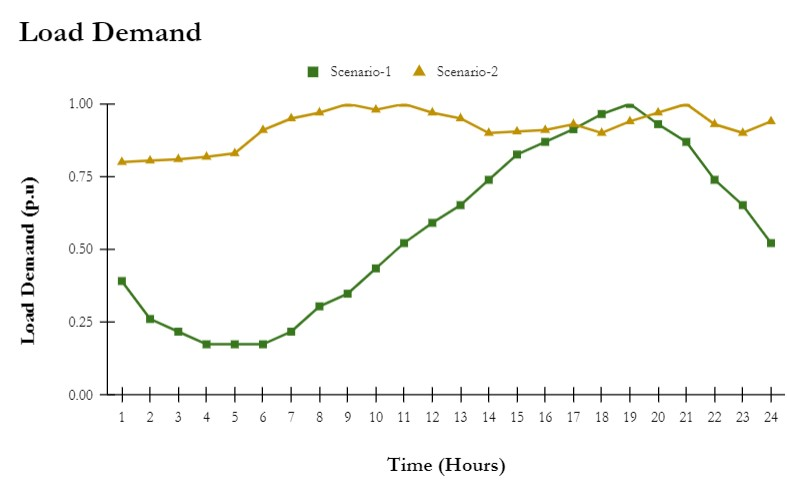
\includegraphics[width=0.7\linewidth]{Figures/load_demand}
			\caption{}
			\label{fig:loaddemand}
		\end{figure}
		

		
	
		
	
	